% Options for packages loaded elsewhere
\PassOptionsToPackage{unicode}{hyperref}
\PassOptionsToPackage{hyphens}{url}
\PassOptionsToPackage{dvipsnames,svgnames,x11names}{xcolor}
%
\documentclass[
  letterpaper,
  DIV=11,
  numbers=noendperiod]{scrartcl}

\usepackage{amsmath,amssymb}
\usepackage{iftex}
\ifPDFTeX
  \usepackage[T1]{fontenc}
  \usepackage[utf8]{inputenc}
  \usepackage{textcomp} % provide euro and other symbols
\else % if luatex or xetex
  \usepackage{unicode-math}
  \defaultfontfeatures{Scale=MatchLowercase}
  \defaultfontfeatures[\rmfamily]{Ligatures=TeX,Scale=1}
\fi
\usepackage{lmodern}
\ifPDFTeX\else  
    % xetex/luatex font selection
\fi
% Use upquote if available, for straight quotes in verbatim environments
\IfFileExists{upquote.sty}{\usepackage{upquote}}{}
\IfFileExists{microtype.sty}{% use microtype if available
  \usepackage[]{microtype}
  \UseMicrotypeSet[protrusion]{basicmath} % disable protrusion for tt fonts
}{}
\makeatletter
\@ifundefined{KOMAClassName}{% if non-KOMA class
  \IfFileExists{parskip.sty}{%
    \usepackage{parskip}
  }{% else
    \setlength{\parindent}{0pt}
    \setlength{\parskip}{6pt plus 2pt minus 1pt}}
}{% if KOMA class
  \KOMAoptions{parskip=half}}
\makeatother
\usepackage{xcolor}
\setlength{\emergencystretch}{3em} % prevent overfull lines
\setcounter{secnumdepth}{-\maxdimen} % remove section numbering
% Make \paragraph and \subparagraph free-standing
\ifx\paragraph\undefined\else
  \let\oldparagraph\paragraph
  \renewcommand{\paragraph}[1]{\oldparagraph{#1}\mbox{}}
\fi
\ifx\subparagraph\undefined\else
  \let\oldsubparagraph\subparagraph
  \renewcommand{\subparagraph}[1]{\oldsubparagraph{#1}\mbox{}}
\fi


\providecommand{\tightlist}{%
  \setlength{\itemsep}{0pt}\setlength{\parskip}{0pt}}\usepackage{longtable,booktabs,array}
\usepackage{calc} % for calculating minipage widths
% Correct order of tables after \paragraph or \subparagraph
\usepackage{etoolbox}
\makeatletter
\patchcmd\longtable{\par}{\if@noskipsec\mbox{}\fi\par}{}{}
\makeatother
% Allow footnotes in longtable head/foot
\IfFileExists{footnotehyper.sty}{\usepackage{footnotehyper}}{\usepackage{footnote}}
\makesavenoteenv{longtable}
\usepackage{graphicx}
\makeatletter
\def\maxwidth{\ifdim\Gin@nat@width>\linewidth\linewidth\else\Gin@nat@width\fi}
\def\maxheight{\ifdim\Gin@nat@height>\textheight\textheight\else\Gin@nat@height\fi}
\makeatother
% Scale images if necessary, so that they will not overflow the page
% margins by default, and it is still possible to overwrite the defaults
% using explicit options in \includegraphics[width, height, ...]{}
\setkeys{Gin}{width=\maxwidth,height=\maxheight,keepaspectratio}
% Set default figure placement to htbp
\makeatletter
\def\fps@figure{htbp}
\makeatother

\KOMAoption{captions}{tableheading}
\makeatletter
\makeatother
\makeatletter
\makeatother
\makeatletter
\@ifpackageloaded{caption}{}{\usepackage{caption}}
\AtBeginDocument{%
\ifdefined\contentsname
  \renewcommand*\contentsname{Table of contents}
\else
  \newcommand\contentsname{Table of contents}
\fi
\ifdefined\listfigurename
  \renewcommand*\listfigurename{List of Figures}
\else
  \newcommand\listfigurename{List of Figures}
\fi
\ifdefined\listtablename
  \renewcommand*\listtablename{List of Tables}
\else
  \newcommand\listtablename{List of Tables}
\fi
\ifdefined\figurename
  \renewcommand*\figurename{Figure}
\else
  \newcommand\figurename{Figure}
\fi
\ifdefined\tablename
  \renewcommand*\tablename{Table}
\else
  \newcommand\tablename{Table}
\fi
}
\@ifpackageloaded{float}{}{\usepackage{float}}
\floatstyle{ruled}
\@ifundefined{c@chapter}{\newfloat{codelisting}{h}{lop}}{\newfloat{codelisting}{h}{lop}[chapter]}
\floatname{codelisting}{Listing}
\newcommand*\listoflistings{\listof{codelisting}{List of Listings}}
\makeatother
\makeatletter
\@ifpackageloaded{caption}{}{\usepackage{caption}}
\@ifpackageloaded{subcaption}{}{\usepackage{subcaption}}
\makeatother
\makeatletter
\@ifpackageloaded{tcolorbox}{}{\usepackage[skins,breakable]{tcolorbox}}
\makeatother
\makeatletter
\@ifundefined{shadecolor}{\definecolor{shadecolor}{rgb}{.97, .97, .97}}
\makeatother
\makeatletter
\makeatother
\makeatletter
\makeatother
\ifLuaTeX
  \usepackage{selnolig}  % disable illegal ligatures
\fi
\IfFileExists{bookmark.sty}{\usepackage{bookmark}}{\usepackage{hyperref}}
\IfFileExists{xurl.sty}{\usepackage{xurl}}{} % add URL line breaks if available
\urlstyle{same} % disable monospaced font for URLs
\hypersetup{
  pdftitle={Assignment},
  pdfauthor={Jan Szczepanek},
  colorlinks=true,
  linkcolor={blue},
  filecolor={Maroon},
  citecolor={Blue},
  urlcolor={Blue},
  pdfcreator={LaTeX via pandoc}}

\title{Assignment}
\author{Jan Szczepanek}
\date{}

\begin{document}
\maketitle
\ifdefined\Shaded\renewenvironment{Shaded}{\begin{tcolorbox}[boxrule=0pt, breakable, interior hidden, sharp corners, frame hidden, borderline west={3pt}{0pt}{shadecolor}, enhanced]}{\end{tcolorbox}}\fi

\renewcommand*\contentsname{Table of contents}
{
\hypersetup{linkcolor=}
\setcounter{tocdepth}{3}
\tableofcontents
}
\begin{figure}

{\centering 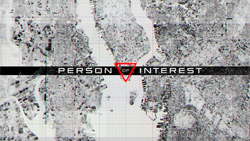
\includegraphics{PoI_files/mediabag/PersonOfInterstLogo.jpg}

}

\caption{Person of Interest Logo from seasons 4-5}

\end{figure}

\hypertarget{description}{%
\subsection{Description}\label{description}}

\emph{Person of Interest} is an American science fiction crime drama
television series that aired on CBS from September 22, 2011, to June 21,
2016. The series was created by Jonathan Nolan, co-writer of \emph{The
Dark Knight} trilogy, and produced by J.J. Abrams. It centers on a
super-intelligent machine that predicts crimes before they happen, and a
team of operatives working to prevent them.

\hypertarget{viewership-summary}{%
\subsection{Viewership Summary}\label{viewership-summary}}

\emph{Person of Interest} premiered to \textbf{13.3 million viewers} and
maintained strong ratings throughout its run. The highest-rated episode
aired in Season 1, while later seasons saw a gradual decline in live
viewership, consistent with overall trends in TV consumption.

\begin{verbatim}
# A tibble: 5 x 3
  Season Year    Avg_Viewers_Millions
   <int> <chr>                  <dbl>
1      1 2011–12                13.3 
2      2 2012–13                14.3 
3      3 2013–14                12.4 
4      4 2014–15                10.6 
5      5 2016                    7.35
\end{verbatim}

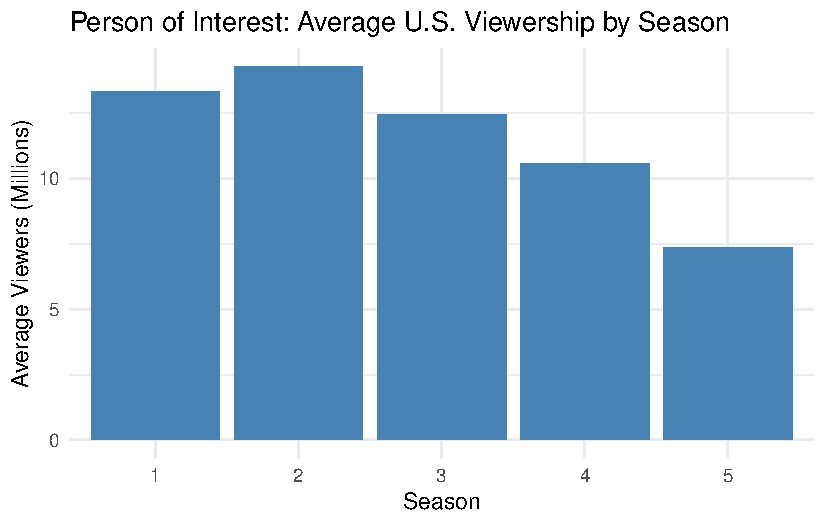
\includegraphics{PoI_files/figure-pdf/unnamed-chunk-1-1.pdf}

\subsubsection{Observations}

\begin{itemize}
\tightlist
\item
  \textbf{Season 1} had a solid start with \textbf{13.3 million} average
  viewers, establishing the show as a strong debut.
\item
  \textbf{Season 2} reached the peak average viewership with
  approximately \textbf{14.28 million viewers}, making it the
  \textbf{5th most-watched} U.S. TV series in the 2012--13 season.
\item
  \textbf{Season 3} saw a moderate dip to \textbf{12.44 million}, still
  keeping the show in a competitive position.
\item
  \textbf{Season 4} remained strong, drawing an average of \textbf{10.58
  million viewers}, and ranked \textbf{21st overall} for the 2014--15
  season.
\item
  \textbf{Season 5} had the \textbf{lowest average viewership}, around
  \textbf{7.35 million viewers}, likely due to a \textbf{shortened
  season (13 episodes)} and a \textbf{shift to summer scheduling}.
\end{itemize}

\subsubsection{Viewership Trends Summary}

The show experienced a notable decrease in viewership over time. For
example, between \textbf{Season 3} and \textbf{Season 5}, the average
audience dropped by \textbf{5.09 million viewers}. Similarly, from
\textbf{Season 2} to \textbf{Season 4}, the show lost around \textbf{3.7
million viewers} on average. These changes reflect the gradual decline
in live broadcast audiences, particularly in later seasons affected by
summer scheduling and shorter episode runs.

\hypertarget{observations-1}{%
\subsubsection{Observations}\label{observations-1}}

\begin{itemize}
\tightlist
\item
  \textbf{Season 1} had a solid start with \textbf{13.3 million} average
  viewers, establishing the show as a strong debut.
\item
  \textbf{Season 2} reached the peak average viewership with
  approximately \textbf{14.28 million viewers}, making it the
  \textbf{5th most-watched} U.S. TV series in the 2012--13 season.
\item
  \textbf{Season 3} saw a moderate dip to \textbf{12.44 million}, still
  keeping the show in a competitive position.
\item
  \textbf{Season 4} remained strong, drawing an average of \textbf{10.58
  million viewers}, and ranked \textbf{21st overall} for the 2014--15
  season.
\item
  \textbf{Season 5} had the \textbf{lowest average viewership}, around
  \textbf{7.35 million viewers}, likely due to a \textbf{shortened
  season (13 episodes)} and a \textbf{shift to summer scheduling}.
\end{itemize}

\hypertarget{viewership-trends-summary-1}{%
\subsubsection{Viewership Trends
Summary}\label{viewership-trends-summary-1}}

The show experienced a notable decrease in viewership over time. For
example, between \textbf{Season 3} and \textbf{Season 5}, the average
audience dropped by \textbf{5.09 million viewers}. Similarly, from
\textbf{Season 2} to \textbf{Season 4}, the show lost around \textbf{3.7
million viewers} on average. These changes reflect the gradual decline
in live broadcast audiences, particularly in later seasons affected by
summer scheduling and shorter episode runs.



\end{document}
